\newpage
\section{QuizziPedia::Back-End}
\label{QuizziPedia::Back-End}
\begin{figure}[ht]
	\centering
	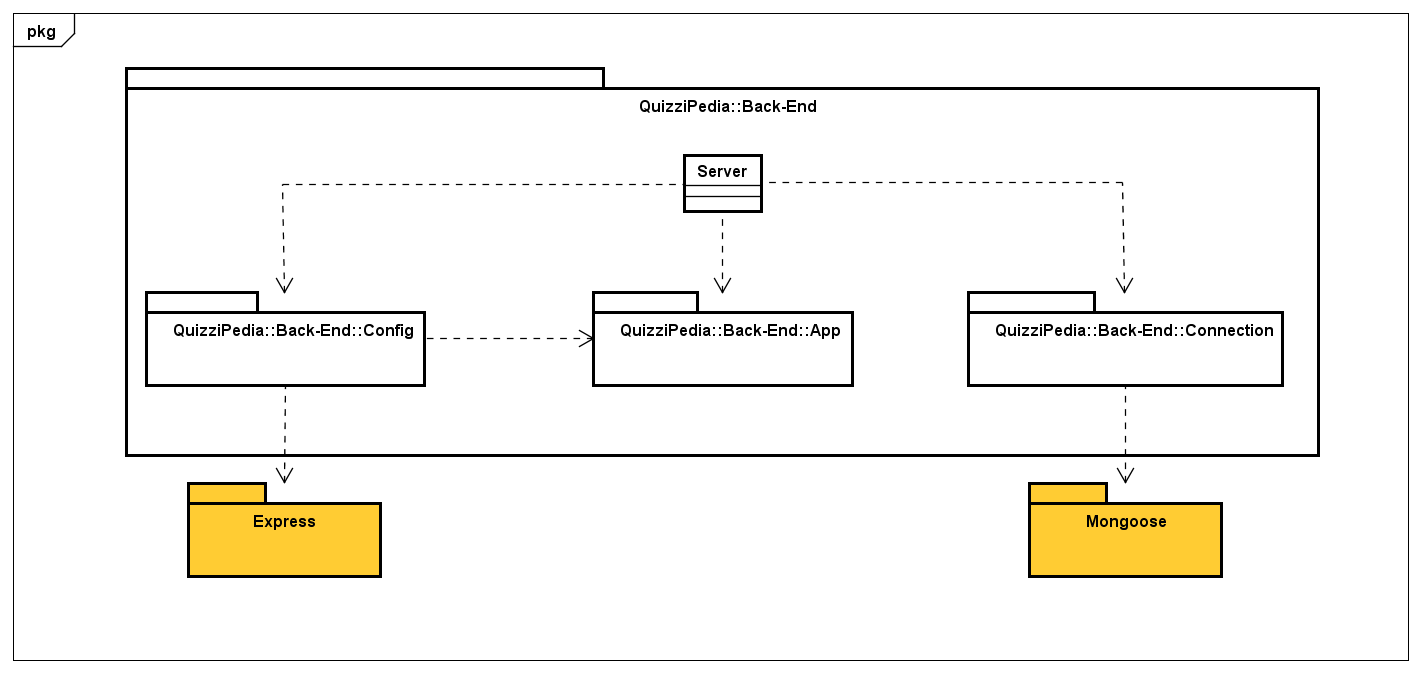
\includegraphics[scale=0.7]{UML/Package/QuizziPedia_Back-End.png}
	\caption{QuizziPedia::Back-End}
\end{figure}
\FloatBarrier
\begin{itemize}
	\item \textbf{Descrizione}:
	\textit{package\ped{G}} contenenti le componenti della parte back-end dell'applicazione;
	\item \textbf{Package contenuti}:
	\begin{itemize}
		\item \texttt{App}:
		\textit{package\ped{G}} contenente le componenti del \textit{server\ped{G}} che implementano il \textit{pattern MVC\ped{G}};
		\item \texttt{Config}:
		\textit{package\ped{G}} contenente le componenti di configurazione del \textit{server\ped{G}}.
	\end{itemize}
\end{itemize}


	

